% listing
\newcommand\pyscript[2]{
\begin{tcolorbox}[width=\linewidth, title=\texttt{#2}]
\lstinputlisting[language=python, firstline=4]{#1/#2}
\end{tcolorbox}
}
\newcommand\txtlst[2]{
\begin{tcolorbox}[width=\linewidth, title=\texttt{#2}]
\lstinputlisting[breaklines=false]{#1/#2}
\end{tcolorbox}
}

% references
\newcommand\figref[1]{Figure~\ref{#1}}

% figures
\newcommand\smallfig[4]{%
\begin{minipage}{0.3333\linewidth}%
\begin{figure}[H]%
\includegraphics[width=\linewidth]{#2/#3.pdf}%
\caption{#4}%
\label{#1}%
\end{figure}%
\end{minipage}%
}
\newcommand\medfig[4]{%
\begin{minipage}{0.5\linewidth}%
\begin{figure}[H]%
\includegraphics[width=\linewidth]{#2/#3.pdf}%
\caption{#4}%
\label{#1}%
\end{figure}%
\end{minipage}%
}
\newcommand\bigfig[4]{
\begin{figure}[H]%
\includegraphics[width=\linewidth]{#2/#3.pdf}%
\caption{#4}%
\label{#1}%
\end{figure}%
}

% data
\newcommand\datdir{../cycle\_report}
\newcommand\res[7]{
\null
\vfill
\subsubsection{#7}\label{#7}
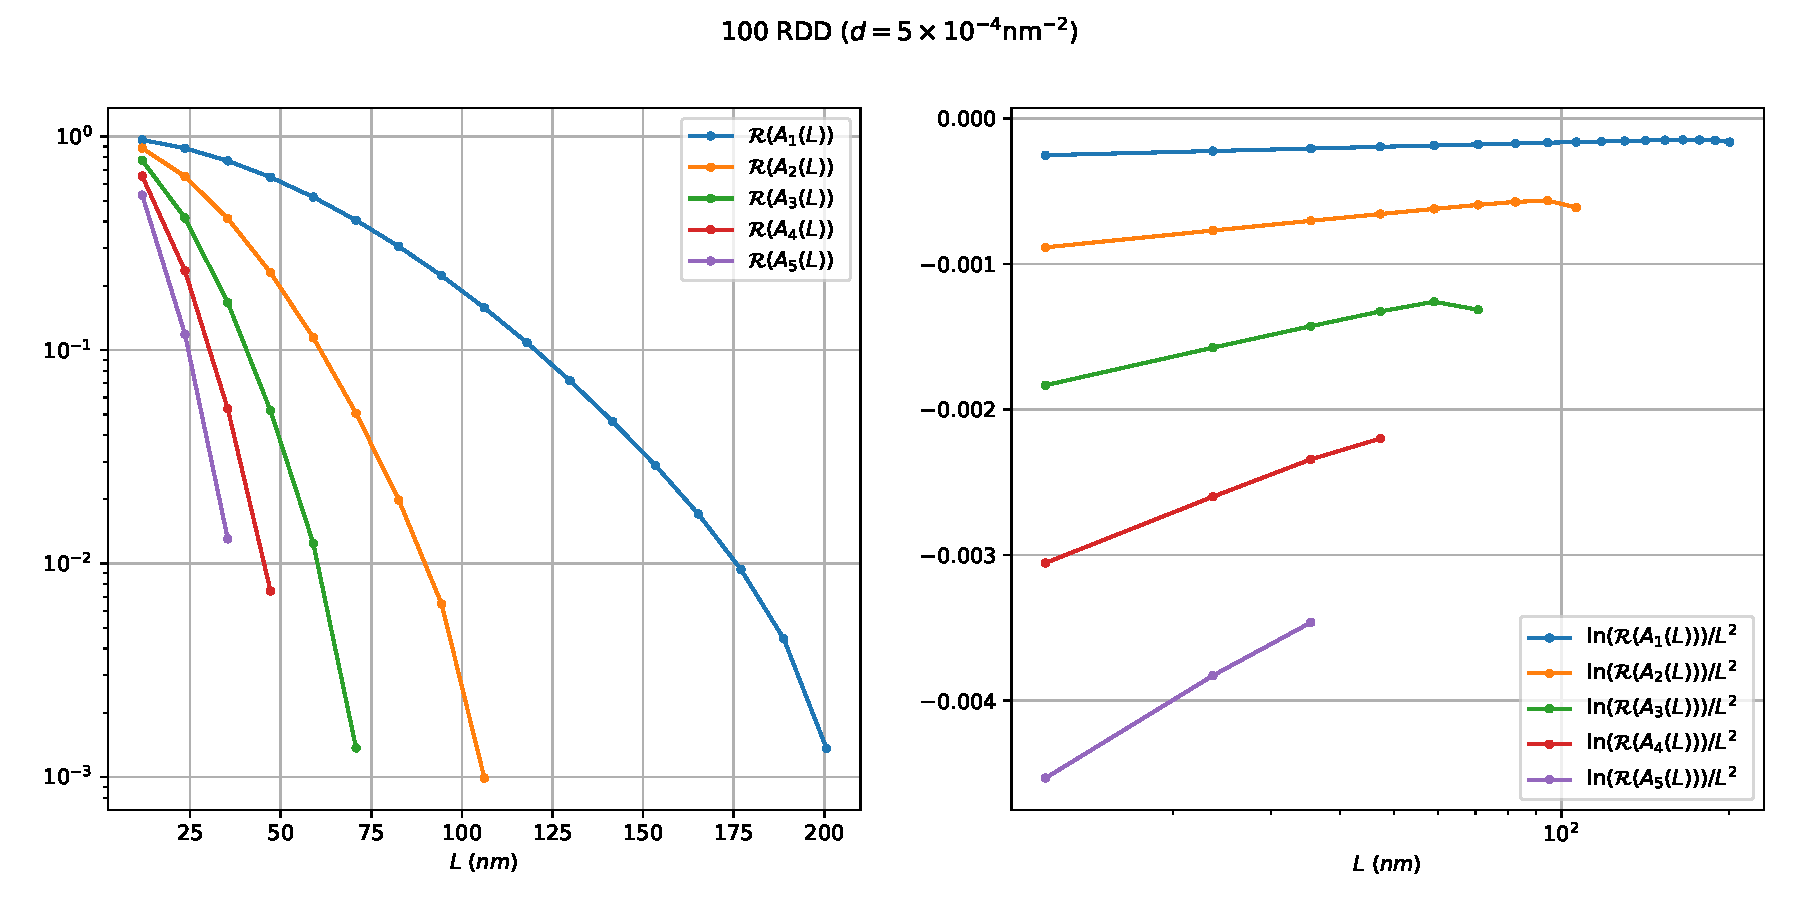
\includegraphics[width=\linewidth]{\datdir/fits_5e#1m-2/#3/output_plot.pdf}
\captionof{figure}{Simulation output}
\begin{center}
\includegraphics[width=0.7\linewidth]{\datdir/maps_5e#1m-2/#2}
\captionof{figure}{Dislocation map}
\end{center}
\includegraphics[width=\linewidth]{\datdir/stats_5e#1m-2/#5}
\includegraphics[width=\linewidth]{\datdir/stats_5e#1m-2/#6}
\captionof{figure}{Spatial analysis}
\columnbreak
}

% maths
\newcommand{\define}[5]{
\ensuremath{#1
\left\{
\begin{array}{ccl}
  #2 &
  \longrightarrow &
  #3 \smallskip \\
  #4 &
  \longmapsto &
  #5
\end{array}
\right.
}
}
\newcommand{\symcircularsegment}{
\begin{picture}(8.5,8)(0,0)
\put(4.25, 3.0){\circle{6}}
\put(0.5, 4.0){\line(1,0){7.5}}
\end{picture}}
\newcommand{\symcirclecircle}{
\begin{picture}(8.5,8)(0,0)
\put(3.5, 3.0){\circle{6}}
\put(5.0, 4.5){\circle{6}}
\end{picture}}
\newcommand{\symcirclesquare}{
\begin{picture}(8.5,8)(0,0)
\put(0.5, 0.0){\line(1,0){5}}
\put(0.5, 0.0){\line(0,1){5}}
\put(0.5, 5.0){\line(1,0){5}}
\put(5.5, 0.0){\line(0,1){5}}
\put(5.0, 4.5){\circle{6}}
\end{picture}}
\newcommand\cirseg{\ensuremath{\gls{area}_{\symcircularsegment}}}
\newcommand\cirsqr{\ensuremath{\gls{area}_{\symcirclesquare}}}
\newcommand\circir{\ensuremath{\gls{area}_{\symcirclecircle}}}
\newcommand\ux{\ensuremath{\overrightarrow{u_x}}}
\newcommand\uy{\ensuremath{\overrightarrow{u_y}}}
\newcommand\uz{\ensuremath{\overrightarrow{u_z}}}
\newcommand\ur{\ensuremath{\overrightarrow{u_r}}}
\newcommand\uphi{\ensuremath{\overrightarrow{u_\varphi}}}

% programs
\newcommand\github[1]{%
\href{https://github.com/DunstanBecht/#1}{\textbf{\color{Blue} \faGithub \color{Blue} \ github.com/DunstanBecht/#1}}%
}
\newcommand\pipinstall[1]{
\begin{tcolorbox}[width=\linewidth, title=shell]
\texttt{pip install -U #1}
\end{tcolorbox}
}
